\section{Introduction}

\subsection{Motivation}

Although the dimuon mass spectrum is well understood in $e^+e^-$ and
$p\bar{p}$ collisions up to collision energies of 0.2 and 2~TeV
respectively, new states may be hidden by
weak couplings to Standard Model particles.  A wide class of
hidden-valley models predicts new states coupling weakly to the
Standard Model yet significantly to a hidden sector, accessible to the
LHC through massive particles that connect the two sectors.  In these
scenarios, massive particles $M$ would be created singly or in pairs
and then decay through the hidden spectrum to the lightest hidden
state: e.g.\ $pp \to M\overline{M}$ and $M \to m X$ where $m$ is the
lightest hidden particle in a cascade chain.  If $m$ is unstable, it would decay with
very small width to the kinematically-accessible Standard Model
states, either democratically ($Z$-like) or to the heaviest accessible
state (Higgs-like).  Muon-pair final states would appear as a
low-mass, high-momentum dimuon resonance, and therefore be collimated
by relativistic boost.  With several low-mass states in the decay
chain, e.g.\ $m_2 \to m_1 m_1 \to 4\mu$, cascades would either produce
two groups of collimated dimuons or one group of four collimated
muons, depending on the boost of $m_2$.  Arbitrarily complex decay
chains are conceivable, and groups of muons might be produced in
association with other Standard Model pairs, such as $e^+e^-$ and
hadrons.  These striking signatures are often called ``lepton jets.''

Hidden, low-mass resonances are especially interesting in light of the
high-energy positron excess reported by the PAMELA primary cosmic-ray
experiment~\cite{Pamela-positron}. While pulsars cannot be conclusively ruled out 
as the source of this excess~\cite{pulsars}, the interstellar positrons could be the
product of WIMP annihilations~\cite{Arkani-Hamed}, assuming that the WIMP annihilation
rate is higher than what would be expected from thermal freeze-out in
the early universe, and also assuming some mechanism to prohibit decay
chains that produce antiprotons, in which no excess was observed.  A
new force boson, $a_{\mbox{\scriptsize dark}}$, with a mass of approximately
1~GeV/$c^2$ and coupling significantly to WIMPs yet weakly to Standard
Model particles, would explain both observations.  Acting as a
long-range Yukawa force, $a_{\mbox{\scriptsize dark}}$ would draw together slow-moving
WIMPs, increasing their effective annihilation cross-section in the
modern era without affecting their production in the early universe. This
mechanism is known as the Sommerfeld enhancement~\cite{Sommerfeld1,Sommerfeld2}.
The lack of an antiproton excess in PAMELA data~\cite{Pamela-proton} can be consistent with
these models if the $a_{\mbox{\scriptsize dark}} \to p\bar{p} X$ channel were
kinematically forbidden~\cite{Arkani-Hamed}; that is, if the mass of $a_{\mbox{\scriptsize dark}}$ 
were below 2~GeV/$c^2$ or so. Alternatively, $a_{\mbox{\scriptsize dark}}$ can have a
preferential coupling to leptons~\cite{mediator-lepton-coupling1,mediator-lepton-coupling2},
which could also explain the annual modulation reported by the DAMA/LIBRA experiment~\cite{Dama}. 
Relatively simple extensions of this picture (see~\cite{Arkani-Hamed} for details), such as adding a dark
Higgs boson $h_{\mbox{\scriptsize dark}}$ to give the $a_{\mbox{\scriptsize dark}}$ its mass, or
introducing the force with non-abelian structure, would produce more
complex event topologies: $2^N$ fermion pairs per lepton jet for a
two-body decay chain with $N$ light states and/or several lepton jets
per event if the decay chain includes heavy particles. These models are particularly natural
in the context of supersymmetry. Depending on the strength of the coupling of the dark sector to 
MSSM, at the LHC one can expect the new signatures to be detectable in MSSM squark/gluino 
production followed by two somewhat different types of cascade decays leading to appearance 
of the dark sector particles. If the coupling is weak, the MSSM cascades proceed in a standard fashion
down to the MSSM LSP, which can then decay to the ```dark photon'' and ``dark neutralino,'' with
the latter being the truly stable dark matter particle~\cite{BaiHan}. If the coupling is strong, one
may expect new large decay channels for squarks into the dark sector particles~\cite{Ruderman}. 
Searches for lepton jets have been performed at D$\O$~\cite{D01,D02} with no observed
signal, but the Tevatron energy may just be too low to access these signals.

Another, very different, motivation derives in the context of Next-to-Minimal Supersymmetric Model (NMSSM)~\cite{Nilles:1982dy,Frere:1983ag,Ellis:1988er,Drees:1988fc,Ellwanger:1993xa,Ellwanger:1995ru,Miller:2003ay},
which extends MSSM by an additional singlet superfield $\langle S \rangle$ in the superpotential. That 
leads to an extension of the Higgs sector compared to MSSM, particularly to the addition of a light higgs boson $a_1$
that can couple of the SM-like Higgs and substantially broaden the phenomenology of the Higgs sector.
Apart from reducing the fine-tuning present in MSSM~\cite{Dermisek:2005ar} and solving the so-called 
``$\mu$--problem''~\cite{mu-problem}, the NMSSM relieves the tension between the low Higgs mass 
predicted by precision electroweak fits and the
direct LEP limit of 114~GeV/$c^2$.  This particular limit assumes that the Higgs
boson decays directly into Standard Model particles with known
branching fractions.  If additional light Higgs bosons allow for
Higgs-to-Higgs decays, the direct limit may be circumvented.  In a
well-defined region of Next-to Minimal SuperSymmetric (NMSSM)
parameter space, the lightest CP-odd Higgs ($a_1$) can have
arbitrarily low mass.  Below the $2m_\tau$ threshold, the branching
fraction for $a_1 \to \mu\mu$ is about 20\%, making its detection in
the muon channel viable at the LHC with already modest amounts of 
data~\cite{Belyaev:nmssm}. For values of the NMSSM parameters that
give the lightest CP-even Higgs ($h_1$) a large singlet field
component, $h_1 \to a_1 a_1$ can be as large as 100\%.  If nature has
chosen this path, the lightest CP-even Higgs mass could be as low as 86~GeV/$c^2$
and the primary light Higgs decay mode could be $h_1 \to a_1 a_1 \to 2\mu,
2\mu$, where the dimuons appear as well-collimated lepton jets. The strongest
constraints on the NMSSM scenarios with light $a_1$ come from LEP~\cite{lep2exclusion}.
Searches at BaBar and CLEO~\cite{cleo-low-ma,babar-low-ma} have little impact
on the allowed parameter space as well as the D\O search for this signature~\cite{Abazov:2009yi}, 
which has only a small impact on the allowed parameter space as it was shown in~\cite{Belyaev:nmssm}.

\subsection{Analysis Strategy}

This analysis is an inclusive, signature-based search for resonant
production of light bosons $m_1$ that decay to pairs of muons (the mass
range searches is from 0.25 to $5$~GeV/$c^2$). To preserve the model independence of the
search, selections are designed to have minimal dependence on the
exact production mechanism of the new bosons, e.g.\ whether they are
produced in electroweak-like processes leading to final states with
isolated dimuons, produced inside hadronic jets, or in cascades of new
particles. The only assumption made in the latter case is that all or
some of the decay chains in the hidden sector reach an on-shell
lowest-mass state $m_1$ before its final decay, as illustrated in
Fig.~\ref{fig:basic_picture}(a). Similarly, selections are designed to
be insensitive to whether $m_1$ decays exclusively to muons or has
other allowed decay channels, e.g.\ $e^+e^-$ or hadron decays. Such model
independence is achieved by avoiding the use of isolation
requirements, which could otherwise severely link acceptances to
the details of the production mechanism and decay branching
fractions. As an illustration, Fig.~\ref{fig:basic_picture}(b) shows a
possible topology where the decay products of two or more spatially
close new bosons overlap, leading to either ``muon jets,'' or ``mixed
jets,'' in which some of the $m_1$ bosons decay to non-muon modes. Finally,
to avoid unnecessary model dependencies, additional objects, such as
isolated single leptons, hadronic jets, and missing energy, are
neither required in the search nor are they forbidden.

\begin{figure}
\mbox{ } \hfill 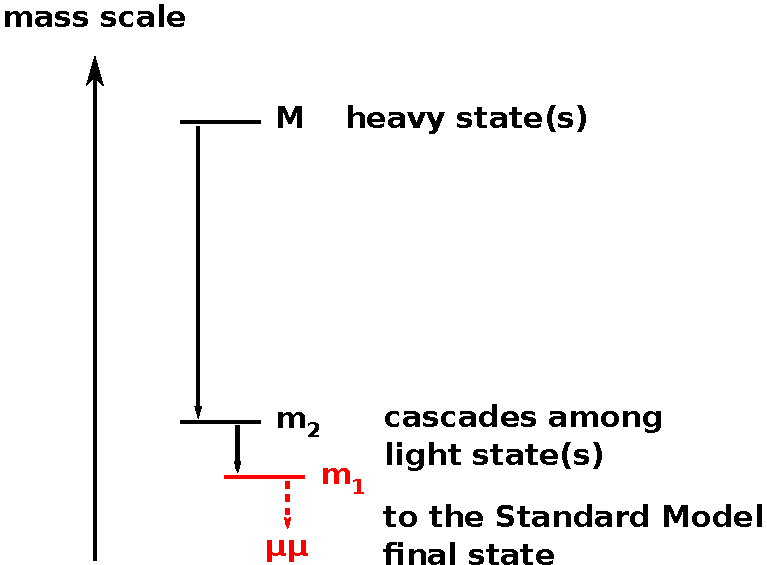
\includegraphics[width=0.45\linewidth]{PLOTS/basic_picture4.pdf} \hfill
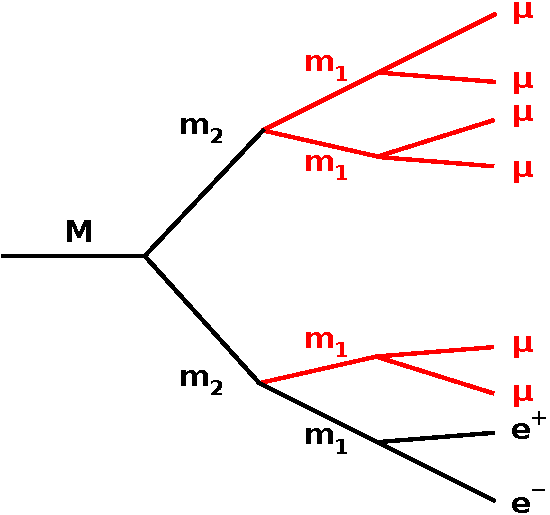
\includegraphics[width=0.35\linewidth]{PLOTS/basic_picture5.pdf} \hfill \mbox{ }
\caption{Schematic of a decay chain from heavy states in the hidden
  sector to light states, ultimately to Standard Model pairs.  We
  identify groups of muons collimated by boost, possibly containing
  non-muons and search for a resonance in muon pairs from $m_1 \to
  \mu\mu$. \label{fig:basic_picture}}
\end{figure}

The strategy of the analysis is to select events with multiple muon
candidates per event, identify the combination of muon pairs most
compatible with the decays of low mass resonances, and search for an
enhancement in the production of muon pairs consistent with the
hypothesis of being the decay products of particles of the same
mass. Here we give an overview of the analysis, full details and definitions are 
provided in the rest of the note. Selection of muon pairs proceeds in two steps. First, 
muons satisfying a minimim-$p_T$ threshold ($p_T>5$ GeV/c) are
iteratively grouped into ``mu-jets'' if a new muon and any oppositely
charged muon in the jet have pairwise invariant mass
$m_{\mu\mu}<9$~GeV/$c^2$.  The procedure continues until all
``mu-jets'' are built.  There is no limit on the number of muons per
group, and not all muons need to be grouped (isolated muons are
allowed). Note that this definition is kinematic, rather than a
geometric based on a $\Delta R$-cone algorithm\footnote{$\Delta R = \sqrt{(\Delta \phi)^2 +
 (\Delta \eta)^2}$}, as was used in the Tevatron searches~\cite{D02}.
The latter leads to unnecessary inefficiencies for resonances of higher 
masses or for pairs produced with a moderate transverse momentum, which
can happen in the dark SUSY $U(1)$ model if mass splitting $\chi_1^0$--$\chi^0_{dark}$ 
is not too large or in the NMSSM as it is  illustrated in Fig.~\ref{fig:openingangle_dr}.

\begin{figure}
\begin{center}
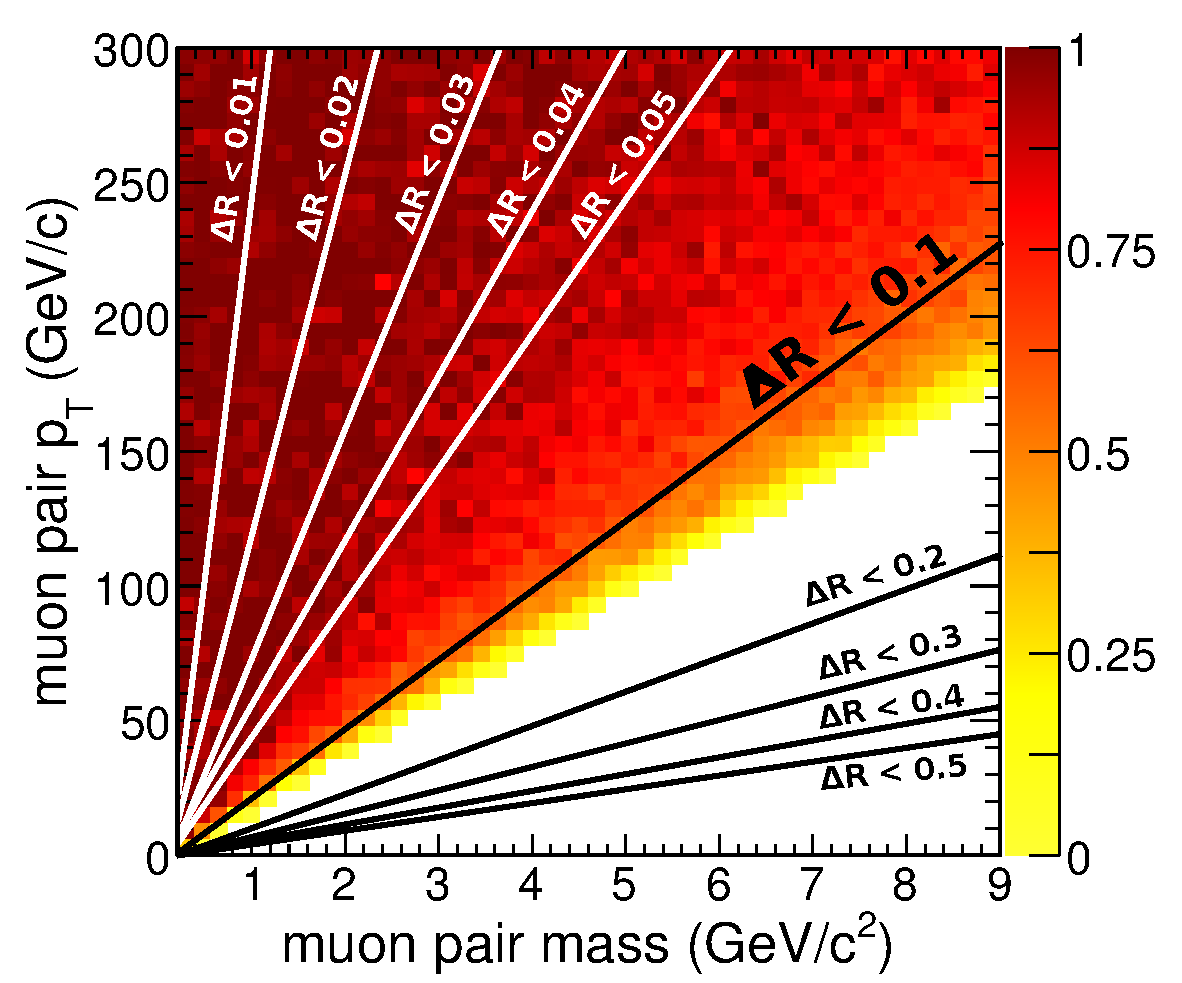
\includegraphics[width=0.65\linewidth]{PLOTS/openingangle_dr.pdf}
\end{center}
\caption{Mass and momentum of dimuons from a toy Monte Carlo (uniform
  in mass, $p_T$, $\eta$ with scalar decays); color scale indicates
  the fraction that pass $\Delta R < 0.1$.  Contour lines are overlaid
  at the center (50\% edges) of similar turn-on curves for a range of
  $\Delta R$ values.\label{fig:openingangle_dr}}
\end{figure}

The second step in the procedure is to classify events by the number of mu-jets
and the number of muons in each mu-jet (if there are other muons in the event not
clustered into mu-jets, they do not affect classification). Next, high-multiplicity mu-jets
are split into a set of electrically neutral muon pairs most consistent with
having a common invariant mass (across all muons clustered in mu-jets in the entire 
event). The best assignment of opposite-sign pairs is preserved for the remainder of the 
analysis and are referred to as ``fundamental dimuons.''  The effectiveness of this simple
procedure is illustrated in Fig.~\ref{fig:four-two-muon-mass} for a
sample signal with a mu-jet containing four muons from $m_2 \to m_1
m_1 \to 4\mu$ ($m_2 = 3$~GeV/$c^2$ and $m_1 = 1$~GeV/$c^2$) by showing
the invariant masses of the selected ``fudamental dimuons'' as well as
the invariant mass of all four muons.

\begin{figure}
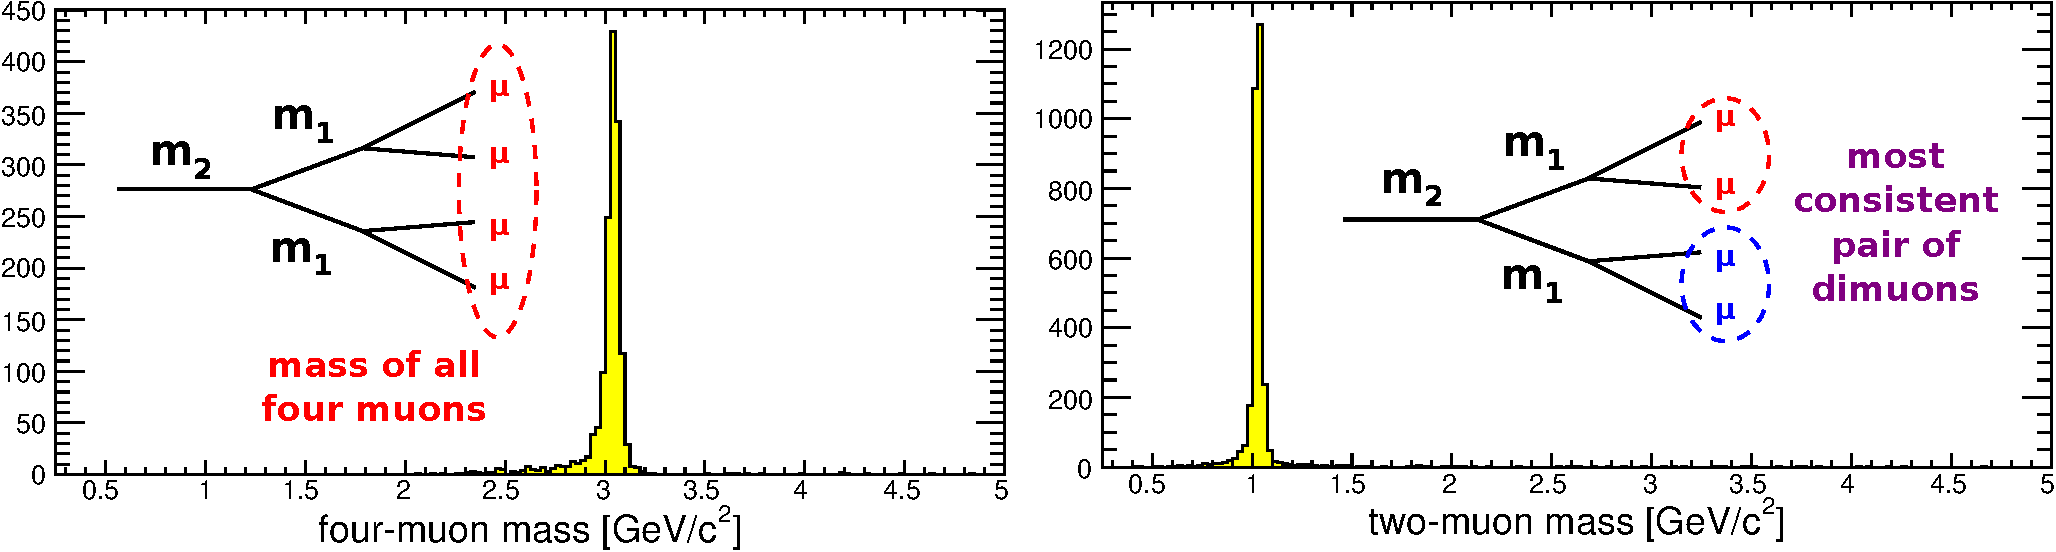
\includegraphics[width=\linewidth]{PLOTS/four-two-muon-mass}
\caption{Identification of fundamental dimuons in a mu-jet containing
  four muons from $m_2 \to m_1 m_1 \to 4\mu$.  The invariant mass of
  all four muons is a sharp peak at $m_2$ (3~GeV/$c^2$ in this
  example), and the invariant mass of the most consistent pair of
  dimuons within this mu-jet is a sharp peak at $m_1$ (1~GeV/$c^2$ in
  this example). \label{fig:four-two-muon-mass}}
\end{figure}

Next, we categorize events based on the number of mu-jets
$N_{\mu-jet}$ and the number of fundamental di-muons in each mu-jet
$N_{\mu\mu}$ as these correspond to different signal topologies and
therefore have different sensitivities to particular models of
interest. These topologies are shown in
Table~\ref{tab:signal_channels}.

\begin{table}[tbh]
\caption{Topologies used to categorize events based on the number of
  mu-jets and the number of muon pairs (fundamental dimuons) in each
  mu-jet.\label{tab:signal_channels}}
\begin{center}
\begin{tabular}{|c|l|l|}
\hline
%\multicolumn{3}{|c|}{hey}\\ \hline
region & Description & Targeted Models \\ \hline
        & \multicolumn{2}{|c|}{$N_{\mu-jet} =1$:}\\ \hline
(a-1) & one dimuon with $p_T > 80$~GeV/$c$ & single high-$p_T$ $m_1 \to \mu\mu$ \\
(a-2) & two fundamental dimuons in a single mu-jet ($4\mu$) & cascades, e.g. $m_2 \to 2 m_1 \to 4\mu$ \\ 
(a-3) & more than four muons in the mu-jet & more complex hierarchy \\ \hline
        & \multicolumn{2}{|c|}{$N_{\mu-jet} =2$:}\\ \hline
(b-1) & both mu-jets contain exactly two muons & heavy $M \to m_1  m_1 \to 4\mu$ \\
         &                                                                   & (e.g. NMSSM Higgs)\\ 
(b-2) & one of the two mu-jets has more than two muons & e.g.\ $M \to m_2 m_1$ or $m_2 m_2$ \\\hline
        & \multicolumn{2}{|c|}{$N_{\mu-jet} \ge 3$:}\\ \hline
(c-1) & $> 2$ mu-jets with any numbers of muons & more complex hierarchy \\
\hline
\end{tabular}
\end{center}
\end{table}

To be explicit, the multi-muon signatures that are excluded from this analysis acceptance are the following:
\begin{itemize}
\item events with no mu-jets (e.g. a $Z \to \mu \mu$ event will not have muons clustered into a mu-jet)
\item events with exactly one mu-jet containing exactly two muons with $p_T < 80$~GeV/$c$ (backgrounds are too high, used as a control sample);
\item events with exactly one mu-jet containing three muons (negligible signal, used as a control sample);
\end{itemize}
As a reminder, any additional ungrouped muons are not counted as mu-jets because a mu-jet requires at least two opposite charged muons in it. A muon would not be grouped if its pairwise invariant mass is greater than 9~GeV/$c^2$ with respect to all other muons of opposite charge in the same vertex.

Events in each category have a fixed number of fundamental dimuons; in
the case of signal events, all such dimuons should have compatible
masses, as they originate from the decays of the same particle type,
while the background events do not have such correlations. For a sample
topology with two or three reconstructed dimuons in the event, this is
schematically illustrated in Figs.~\ref{fig:diagonal}(a) and (b), respectively. The signal,
if observed, will be somewhere on the diagonal while the backgrounds will be distributed
across the entire multi-dimensional space. Known resonances may form an enhancement
near the diagonal, but those will also appear as vertical or horizontal acceptances in
events that have only one of the dimuons coming from a resonance. We therefore analyze the
$N_{\mu\mu}$-dimensional distribution of fundamental dimuon masses for
each category and search for an enhancement near the diagonal. In some
of the topologies, one could also analyze the invariant mass
distributions for groups of fundamental dimuons in the same mu-jet to
search for a possible hierarchial structure of the hidden sector. To
avoid overcomplicating the interpretation of our results, we decided
to base the main results on an analysis of the
$N_{\mu\mu}$-dimensional space of fundamental dimuon masses
alone. However, if an excess is observed, we will perform an
additional analysis, searching for possible structure in the spectrum
of new particles.

The analysis of the multi-dimensional spectra is performed using a
binned likelihood fit with the background shape determined from
properly defined background-enriched samples and a Crystal Ball shape
used to model the signal. For multi-dimuon topologies, the fit is
performed in the region near the diagonal, while the normalization for background
is determined from the fit in the side-band (off-diagonal) region. For single-dimuon topologies, a fit with
floating signal and background normalizations is used. The posterior for
the signal normalization is used to either discover or set limits on the
production rate of new resonances. 

\begin{figure}
\begin{center}
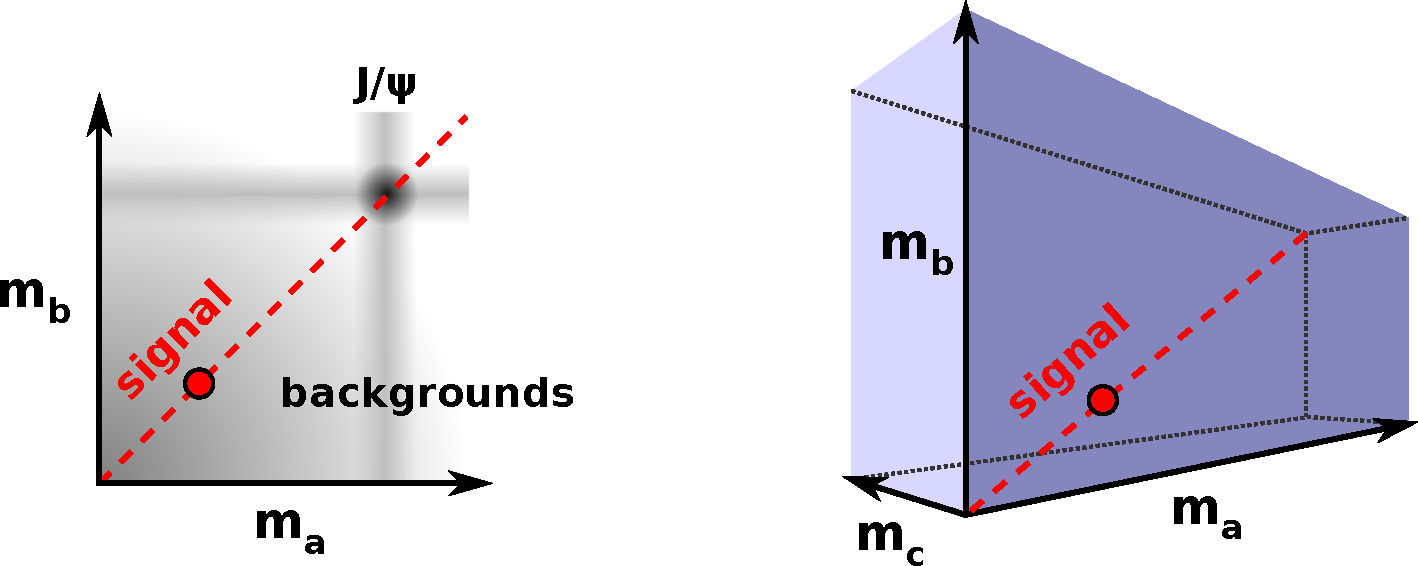
\includegraphics[width=0.75\linewidth]{PLOTS/diagonal.pdf}
\end{center}
\caption{Schematic of multi-dimensional search for signal in topologies with two (a) and three (b) dimuons
in the event.  The signal, if observed, will appear as a peak 
somewhere on the diagonal while the backgrounds events will have a distribution 
spread across the entire multi-dimensional space. Known resonances may form an enhancement
near the diagonal, but those will also appear as vertical or horizontal enhancements in
events that have only one of the dimuons coming from a resonance. \label{fig:diagonal}}
\end{figure}
